% !TeX program = pdflatex
\documentclass[11pt]{article}

% --- arXiv-compatible packages ---
\usepackage[utf8]{inputenc}
\usepackage[T1]{fontenc}
\usepackage{microtype}
\usepackage{amsmath,amssymb,amsfonts}
\usepackage{graphicx}
\usepackage{booktabs}
\usepackage{multirow}
\usepackage{hyperref}
\usepackage{xcolor}
\usepackage{enumitem}
\usepackage[margin=1in]{geometry}
\usepackage{caption}
\usepackage{subcaption}
\usepackage{natbib}
\bibliographystyle{plainnat}

\hypersetup{
    colorlinks=true,
    linkcolor=blue!70!black,
    citecolor=blue!70!black,
    urlcolor=blue!70!black
}

% --- Custom commands ---
\newcommand{\talkex}{\textsc{TalkEx}}
\newcommand{\macrof}{Macro-F1}
\newcommand{\pp}{\,pp}

\title{%
\talkex{}: A Hybrid Cascaded Architecture for\\
Conversation Intent Classification\\[6pt]
\large Combining BM25, Frozen Embeddings, and Deterministic Rules\\
over Multi-Turn PT-BR Customer Service Conversations%
}

\author{%
Paulo Henrique Vieira Nascimento\thanks{MSc candidate, MIT Media Lab (Conversation Intelligence Group). Correspondence: \texttt{paulohenriquevn@gmail.com}}
}

\date{March 2026}

\begin{document}
\maketitle

% ============================================================================
% ABSTRACT
% ============================================================================
\begin{abstract}
We present \talkex{}, a modular NLP pipeline for intent classification in Brazilian Portuguese customer service conversations. \talkex{} combines three paradigms that are typically studied in isolation: BM25 lexical retrieval, frozen multilingual sentence embeddings (\texttt{paraphrase-multilingual-MiniLM-L12-v2}, 384 dimensions), and a deterministic semantic rule engine compiled from a domain-specific language (DSL) into typed abstract syntax trees (ASTs). We evaluate four hypotheses on a post-audit corpus of 2,122 PT-BR conversations spanning 8 intent classes, using 5 random seeds and Wilcoxon signed-rank tests. \textbf{H1} (hybrid retrieval): confirmed --- Hybrid-LINEAR achieves MRR\,=\,0.853 vs.\ BM25 0.835 ($p$\,=\,0.017, $r$\,=\,0.29). \textbf{H2} (combined features): confirmed --- lexical+embedding LightGBM achieves \macrof{}\,=\,0.722 vs.\ lexical-only 0.334 ($p$\,$<$\,$10^{-35}$, $r$\,=\,0.84). \textbf{H3} (rule integration): inconclusive --- rules-as-features yield \macrof{}\,=\,0.740 vs.\ ML-only 0.722 ($+1.8\pp$, $p$\,=\,0.131), while rules-as-override \emph{degrades} performance ($p$\,$<$\,$10^{-4}$). \textbf{H4} (cascaded inference): refuted --- a structural cost inversion makes the cascade more expensive than the uniform pipeline. An ablation study quantifies component contributions: embeddings $+33.0\pp$, lexical $+2.9\pp$, rules $+1.8\pp$, structural $+1.3\pp$. LightGBM classification trains in $\sim$6 seconds on CPU with no encoder fine-tuning; embedding generation leverages GPU acceleration on Google Colab (Tesla T4), demonstrating that competitive intent classification is achievable on freely available cloud infrastructure.

\medskip
\noindent\textbf{Keywords:} hybrid retrieval, intent classification, BM25, sentence embeddings, rule engine, Brazilian Portuguese, customer service, conversation intelligence
\end{abstract}

% ============================================================================
% 1. INTRODUCTION
% ============================================================================
\section{Introduction}
\label{sec:intro}

Customer service operations in Brazil generate millions of conversations per month across voice, chat, email, and social media channels. Industry estimates indicate that fewer than 5\% of these conversations receive analytical treatment beyond manual agent disposition codes --- a categorization widely recognized as inconsistent and coarse-grained. The remaining 95\% persists as unstructured data, inaccessible to search, classification, or trend analysis at scale.

This analytical gap has concrete consequences: compliance teams cannot audit agent behavior at scale, churn signals spanning multiple turns go undetected, and quality assurance depends on unreliable self-reported codes. Automated conversation intelligence systems that classify intents, retrieve similar interactions, and produce auditable evidence for each decision would directly address these operational needs.

Three NLP paradigms offer complementary capabilities for this task:

\begin{enumerate}[leftmargin=*,itemsep=2pt]
    \item \textbf{Lexical retrieval} (BM25) excels at exact term matching --- product names, regulatory keywords, cancellation verbs --- but fails on paraphrases and implicit intent.
    \item \textbf{Dense embeddings} from pretrained sentence encoders capture semantic similarity and paraphrase invariance, but struggle with domain-specific vocabulary and exact term matching.
    \item \textbf{Deterministic rules} provide controllable precision and auditable evidence for known patterns, but cannot generalize beyond their lexical coverage.
\end{enumerate}

These paradigms are predominantly studied in isolation. Hybrid retrieval work focuses on passage retrieval benchmarks in English \citep{formal2021splade,khattab2020colbert,karpukhin2020dense}. Embedding-based classification typically fine-tunes encoders \citep{tunstall2022setfit,reimers2019sentencebert}. Rule engines are either standalone or fully replaced by neural systems. The integration of all three within a unified pipeline, evaluated on multi-turn conversational data in a non-English language, remains unexplored.

\talkex{} addresses this gap. We propose a modular cascaded architecture that combines BM25, frozen multilingual embeddings, supervised classification (LightGBM), and a DSL-compiled semantic rule engine. We evaluate four hypotheses on a 2,122-record PT-BR customer service corpus across 8 intent classes:

\begin{description}[leftmargin=0.5cm,itemsep=2pt]
    \item[H1] Hybrid retrieval (BM25 + ANN) outperforms isolated retrieval in MRR.
    \item[H2] Combined lexical + embedding features outperform lexical-only features in \macrof{}.
    \item[H3] Deterministic rules complement ML classification.
    \item[H4] Cascaded inference reduces computational cost without quality loss.
\end{description}

Our contributions are: (1) empirical evidence of hybrid retrieval complementarity in the PT-BR conversational domain; (2) competitive intent classification (\macrof{}\,=\,0.722) without fine-tuning, training in $\sim$6 seconds on Google Colab; (3) the first empirical comparison of three rule integration strategies (features, override, standalone) within a unified conversational pipeline; (4) an honest negative result on cascaded inference, with structural analysis of why the cost model fails; and (5) \talkex{}, an open-source framework implementing the complete pipeline with 1,883+ automated tests.


% ============================================================================
% 2. RELATED WORK
% ============================================================================
\section{Related Work}
\label{sec:related}

\paragraph{Hybrid Retrieval.} The complementarity of lexical and semantic signals has been validated across multiple benchmarks. SPLADE \citep{formal2021splade} learns sparse representations from MLM heads; ColBERT \citep{khattab2020colbert} introduces late interaction via token-level matching; DPR \citep{karpukhin2020dense} trains bi-encoders on question-passage pairs. \citet{rayo2025hybrid} provide the closest methodological precedent, achieving Recall@10\,=\,0.833 with hybrid BM25 + BGE fusion on regulatory texts ($\alpha$\,=\,0.65). However, their corpus is formal English regulatory text --- structurally different from informal multi-turn PT-BR conversations. \citet{harris2024bm25} demonstrate that BM25 outperforms off-the-shelf semantic models on structured medical documents, reinforcing the ``always benchmark BM25 first'' principle.

\paragraph{Embedding-Based Classification.} \citet{reimers2019sentencebert} demonstrated that contrastively trained sentence encoders produce meaningful similarity spaces. SetFit \citep{tunstall2022setfit} achieves competitive few-shot classification using sentence embeddings. The ``embeddings represent, classifiers decide'' paradigm \citep{anthusai2024embeddings} separates representation from decision-making. Most prior work fine-tunes encoders; using a \emph{frozen} multilingual encoder with gradient-boosted trees on PT-BR is, to our knowledge, novel.

\paragraph{Rule-Based NLP.} SystemT \citep{chiticariu2013systemT} demonstrated industrial-scale rule-based extraction. Snorkel \citep{ratner2017snorkel} uses labeling functions as weak supervision. Production engines (Rasa, Dialogflow) support rules but do not integrate them as soft ML features. The soft integration of DSL-compiled rules as classifier features (rather than hard overrides) is a novel contribution.

\paragraph{Conversational Intent Classification.} Standard benchmarks (CLINC150, BANKING77) are English, single-turn, and single-utterance. Multi-turn intent modeling \citep{zhang2021multi} and attention-based classification \citep{lyu2025attention} address richer context but remain English-focused. PT-BR conversational intent classification is virtually unexplored.

\paragraph{Portuguese NLP.} BERTimbau \citep{souza2020bertimbau} provides PT-BR BERT, but no public multi-turn customer service dataset with intent annotations existed before this work.


% ============================================================================
% 3. TALKEX ARCHITECTURE
% ============================================================================
\section{\talkex{} Architecture}
\label{sec:architecture}

\talkex{} implements a multi-stage NLP pipeline with cascaded processing:

\begin{enumerate}[leftmargin=*,itemsep=2pt]
    \item \textbf{Ingestion \& Turn Segmentation.} Raw conversations are parsed, speaker-attributed, and segmented into turns using the \texttt{TurnSegmenter}.
    \item \textbf{Context Window Construction.} A \texttt{SlidingWindowBuilder} generates overlapping 5-turn windows (stride 2), capturing multi-turn dependencies.
    \item \textbf{Text Normalization.} Unicode NFD decomposition removes diacritics; case folding ensures ``n\~{a}o'' and ``nao'' match. Critical for PT-BR.
    \item \textbf{Embedding Generation.} \texttt{paraphrase-multilingual-MiniLM-L12-v2} (384 dims, frozen) generates turn-level and window-level embeddings via mean pooling.
    \item \textbf{Hybrid Retrieval.} BM25 (via \texttt{rank-bm25}) and ANN (via FAISS flat index) produce independent top-$K$ candidate lists, fused via linear interpolation: $S = \alpha \cdot s_{\text{BM25}} + (1-\alpha) \cdot s_{\text{ANN}}$.
    \item \textbf{Classification.} LightGBM (100 estimators, 31 leaves) trained on concatenated features: TF-IDF (7 dims), BM25 scores (2 dims), structural metadata (4 dims), 384-dim embeddings, and binary rule activation flags (2 dims). Total: 397 features for the full pipeline.
    \item \textbf{Semantic Rule Engine.} A DSL is compiled to typed ASTs supporting lexical predicates (\texttt{contains\_any}, \texttt{regex}), semantic predicates (\texttt{intent\_score}, \texttt{embedding\_similarity}), structural predicates (\texttt{speaker}, \texttt{channel}), and contextual predicates (\texttt{repeated\_in\_window}). Every rule execution produces traceable evidence.
    \item \textbf{Window-to-Conversation Aggregation.} Per-window class probabilities are averaged; the final label is determined by argmax over the mean distribution.
\end{enumerate}

\noindent\textbf{Design Axioms.} \emph{Embeddings represent, classifiers decide} --- cosine similarity is never treated as classification. \emph{Always benchmark BM25} before semantic approaches. \emph{LLMs offline only} --- lightweight models for online inference. \emph{Every prediction carries evidence} --- label, score, confidence, threshold, model version, and text evidence.


% ============================================================================
% 4. EXPERIMENTAL SETUP
% ============================================================================
\section{Experimental Setup}
\label{sec:setup}

\subsection{Dataset}

We use the \texttt{RichardSakaguchiMS/brazilian-customer-service-conversations} dataset (HuggingFace, Apache 2.0), expanded with controlled synthetic generation (Claude Sonnet, offline batch). A comprehensive data audit removed 135 records (duplicates, few-shot contamination, ambiguous labels), consolidating the taxonomy from 9 to 8 intent classes by eliminating \texttt{outros}. Human review confirmed $\geq$96.7\% label accuracy.

\begin{figure}[t]
    \centering
    
\includegraphics[width=\linewidth]{fig_dataset_distribution.pdf}
    \caption{Post-audit corpus: 2,122 conversations across 8 intent classes. (a) Overall class distribution showing natural imbalance (reclamacao 17.3\% to elogio 6.9\%). (b) Stratified train/val/test splits preserving class proportions.}
    \label{fig:dataset}
\end{figure}

The post-audit corpus comprises 2,122 conversations (847 original + 1,275 synthetic) with 8 intent classes: \textit{cancelamento} (213), \textit{compra} (238), \textit{duvida\_produto} (340), \textit{duvida\_servico} (334), \textit{elogio} (147), \textit{reclamacao} (368), \textit{saudacao} (172), and \textit{suporte\_tecnico} (310). Figure~\ref{fig:dataset} shows the distribution.

\subsection{Protocol}

All experiments use 5 random seeds [13, 42, 123, 2024, 999] with stratified 70/15/15\% train/val/test splits at the \emph{conversation level} (preventing window-level leakage). Results are reported as mean $\pm$ std across seeds. Statistical significance is assessed via Wilcoxon signed-rank tests ($\alpha$\,=\,0.05) with bootstrap 95\% CIs (10,000 resamples). Effect sizes are reported as $r = Z/\sqrt{N}$.

\subsection{Metrics}

\textbf{H1:} MRR (primary), Recall@$K$, nDCG@$K$ for $K \in \{5, 10, 20\}$. \textbf{H2/H3:} \macrof{} (primary), per-class F1, accuracy. \textbf{H4:} Cost per window (ms), $\Delta$F1, \% resolved per stage.

\subsection{Infrastructure}

All experiments were executed on Google Colab with a Tesla T4 GPU (15\,GB VRAM). Embedding generation leverages GPU acceleration via PyTorch/CUDA; LightGBM classification trains on CPU ($\sim$6 seconds). The full experiment suite completes in under 1 hour. Software: Python 3.11+, sentence-transformers, scikit-learn, LightGBM, FAISS (cpu), rank-bm25. The \talkex{} codebase includes 1,883+ automated tests.


% ============================================================================
% 5. RESULTS
% ============================================================================
\section{Results}
\label{sec:results}

% --- H1 ---
\subsection{H1: Hybrid Retrieval (Confirmed)}

\begin{figure}[t]
    \centering
    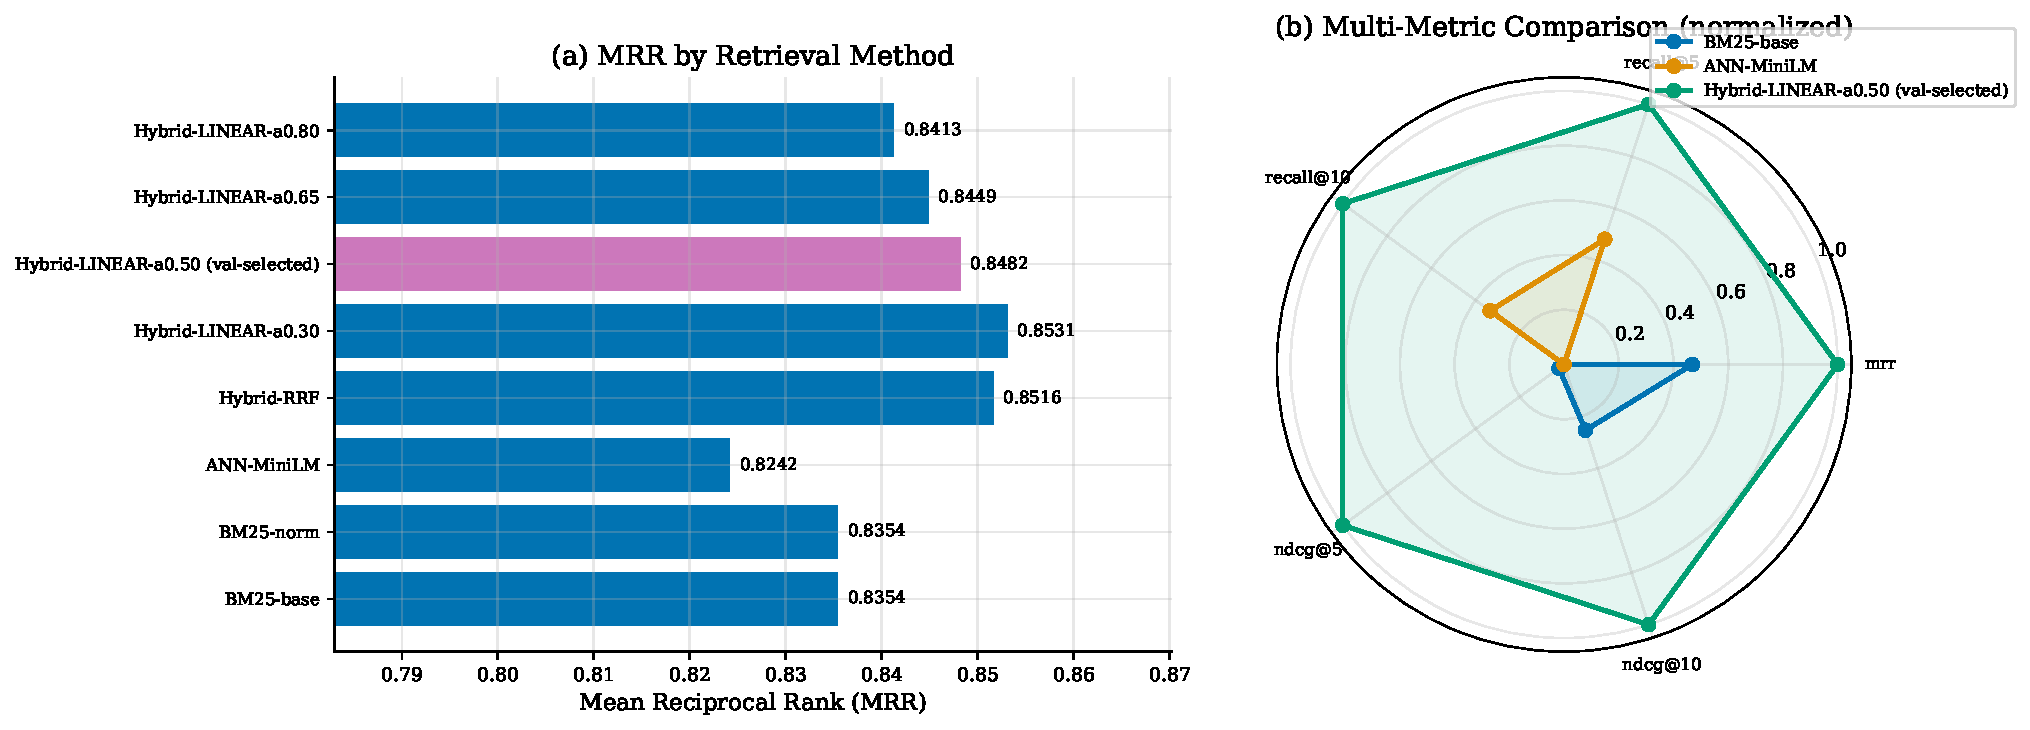
\includegraphics[width=\linewidth]{fig_h1_retrieval.pdf}
    \caption{H1 results. (a) MRR comparison across 8 retrieval variants. Hybrid-LINEAR-$\alpha$0.30 achieves the highest MRR (0.853). (b) Radar chart showing multi-metric profile for BM25, ANN, and the best hybrid variant.}
    \label{fig:h1}
\end{figure}

Table~\ref{tab:h1} and Figure~\ref{fig:h1} present the H1 results. The best hybrid configuration (Hybrid-LINEAR, $\alpha$\,=\,0.30, weighting BM25 at 30\% and ANN at 70\%) achieves MRR\,=\,0.853, significantly outperforming both BM25-base (MRR\,=\,0.835, $p$\,=\,0.017, $r$\,=\,0.29, 95\% CI [0.003, 0.033]) and pure ANN (MRR\,=\,0.824, $p$\,=\,0.030). No significant differences were found between hybrid variants with different $\alpha$ values, nor between linear fusion and RRF, suggesting robustness to moderate hyperparameter variation.

\begin{table}[t]
\centering
\caption{H1: Retrieval system comparison (MRR, primary metric).}
\label{tab:h1}
\small
\begin{tabular}{@{}llccc@{}}
\toprule
\textbf{System} & \textbf{Category} & \textbf{MRR} & \textbf{nDCG@10} & \textbf{Recall@10} \\
\midrule
BM25-base        & Lexical  & 0.835 & 0.632 & 0.037 \\
BM25-norm         & Lexical  & 0.835 & 0.632 & 0.037 \\
ANN-MiniLM        & Semantic & 0.824 & 0.625 & 0.038 \\
\midrule
Hybrid-RRF        & Hybrid   & 0.852 & 0.653 & 0.039 \\
Hybrid-LINEAR-$\alpha$0.30 & Hybrid & \textbf{0.853} & 0.648 & 0.038 \\
Hybrid-LINEAR-$\alpha$0.50 & Hybrid & 0.848 & 0.651 & 0.039 \\
Hybrid-LINEAR-$\alpha$0.65 & Hybrid & 0.845 & 0.648 & 0.039 \\
Hybrid-LINEAR-$\alpha$0.80 & Hybrid & 0.841 & 0.638 & 0.038 \\
\bottomrule
\end{tabular}
\end{table}

The optimal $\alpha$\,=\,0.30 (BM25 weight) differs from the 0.65 reported by \citet{rayo2025hybrid} for regulatory texts, suggesting that informal conversational text benefits more from semantic signals than formal regulatory language. \textbf{H1 is confirmed.}

% --- H2 ---
\subsection{H2: Combined Features (Confirmed)}

\begin{figure}[t]
    \centering
    
\includegraphics[width=\linewidth]{fig_h2_classification.pdf}
    \caption{H2 results. (a) Heatmap of \macrof{} across feature sets and classifiers. Adding embeddings doubles or triples \macrof{} across all classifiers. (b) Best lexical-only (0.334) vs.\ best lexical+embedding (0.722): $+$0.387 gain.}
    \label{fig:h2}
\end{figure}

\begin{figure}[t]
    \centering
    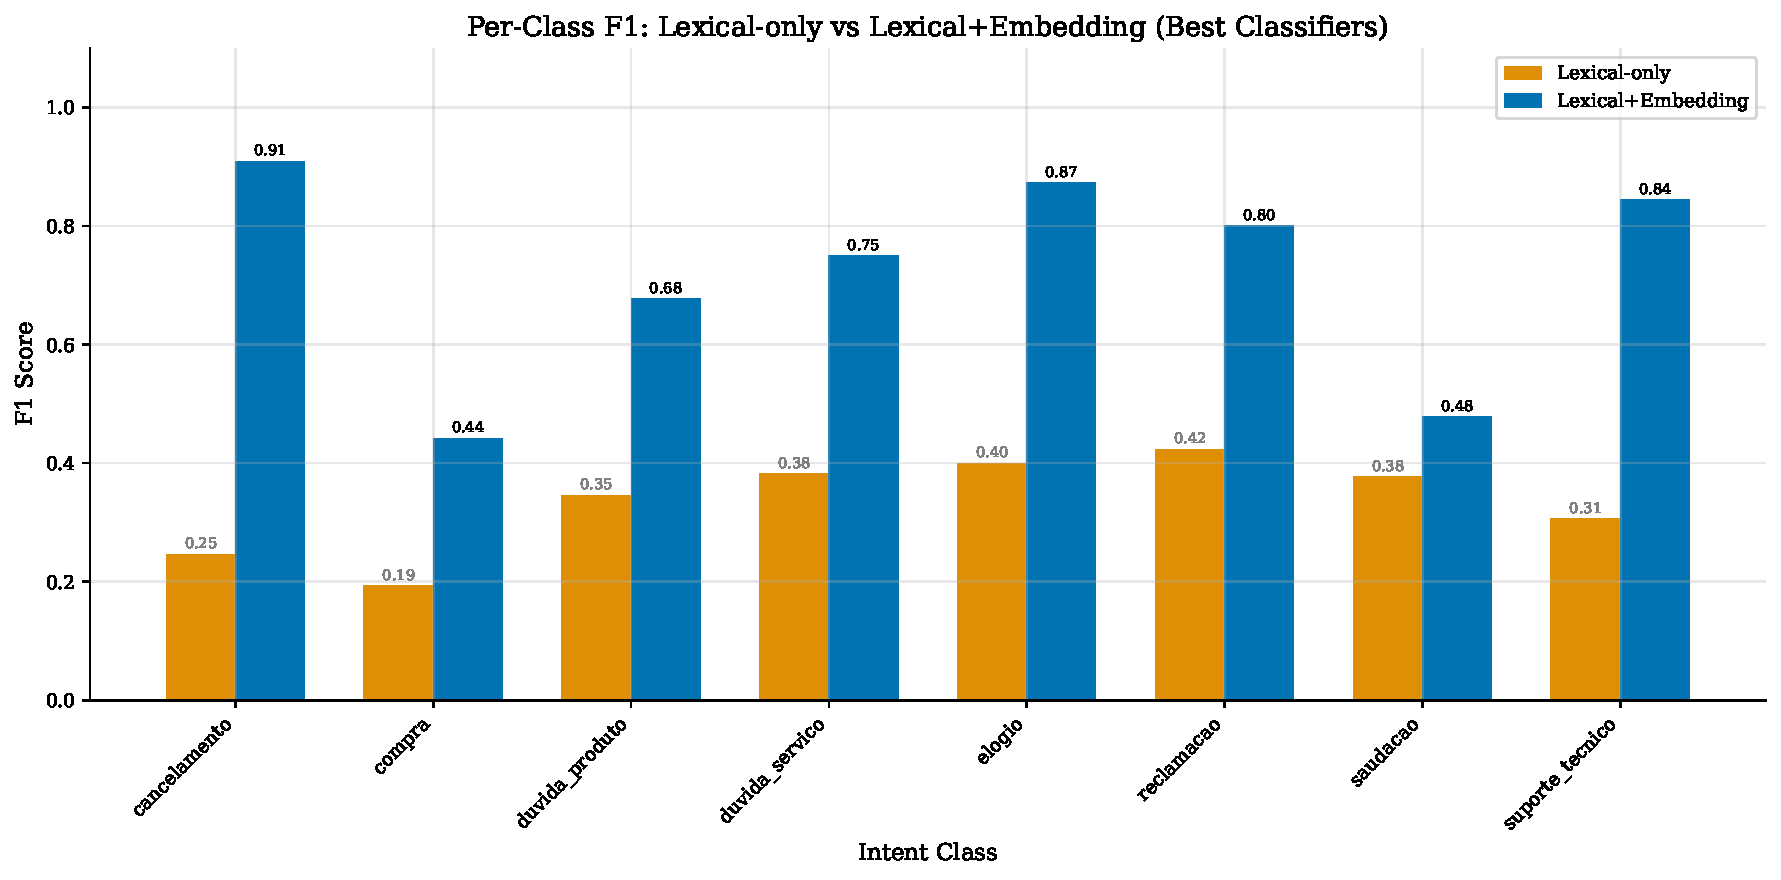
\includegraphics[width=\linewidth]{fig_h2_per_class.pdf}
    \caption{Per-class F1 comparison: lexical-only (LightGBM) vs.\ lexical+embedding (LightGBM). Gains are universal across all 8 classes, largest for semantically diffuse intents (cancelamento $+$0.66, elogio $+$0.47).}
    \label{fig:h2_perclass}
\end{figure}

Table~\ref{tab:h2} and Figures~\ref{fig:h2}--\ref{fig:h2_perclass} present the H2 results. Combining lexical features with 384-dim frozen embeddings yields dramatic improvements across all three classifier families. The best configuration (lexical+emb LightGBM, \macrof{}\,=\,0.722) outperforms the best lexical-only (LightGBM, \macrof{}\,=\,0.334) by $+38.7\pp$ ($p < 10^{-35}$, $r$\,=\,0.84, large effect).

\begin{table}[t]
\centering
\caption{H2: \macrof{} across feature sets and classifiers.}
\label{tab:h2}
\small
\begin{tabular}{@{}lccc@{}}
\toprule
\textbf{Feature Set} & \textbf{LogReg} & \textbf{LightGBM} & \textbf{MLP} \\
\midrule
Lexical-only        & 0.201 & 0.334 & 0.105 \\
Lexical+Embedding   & 0.610 & \textbf{0.722} & 0.620 \\
\midrule
$\Delta$ (gain)     & $+$0.409 & $+$0.387 & $+$0.515 \\
\bottomrule
\end{tabular}
\end{table}

Per-class analysis (Figure~\ref{fig:h2_perclass}) reveals that gains are consistent across all 8 classes, with the largest improvements on intents that resist lexical enumeration: \textit{cancelamento} ($+$0.66), \textit{suporte\_tecnico} ($+$0.53), \textit{elogio} ($+$0.47). The smallest gain is on \textit{saudacao} ($+$0.10), the most lexically regular class. This pattern is consistent with the theoretical expectation that dense embeddings benefit semantically diffuse classes most. \textbf{H2 is confirmed.}

% --- H3 ---
\subsection{H3: Rule Integration (Inconclusive)}

\begin{figure}[t]
    \centering
    
\includegraphics[width=\linewidth]{fig_h3_rules.pdf}
    \caption{H3 results. (a) \macrof{} across rule integration strategies. Rules-as-features (0.740) slightly exceeds ML-only (0.722), but rules-as-override (0.680) \emph{degrades} performance. (b) Per-class comparison showing ML-only vs.\ ML+Rules-feature.}
    \label{fig:h3}
\end{figure}

Table~\ref{tab:h3} and Figure~\ref{fig:h3} present the H3 results. The rules-as-features strategy achieves \macrof{}\,=\,0.740 vs.\ ML-only 0.722, a difference of $+1.8\pp$. The Wilcoxon test returns $p$\,=\,0.131 with 95\% CI [$-$0.004, $+$0.039], which includes zero. The positive direction is consistent but statistically inconclusive.

\begin{table}[t]
\centering
\caption{H3: Rule integration strategies. Only 2 lexical rules were tested (\texttt{rule\_cancel}, \texttt{rule\_complaint}).}
\label{tab:h3}
\small
\begin{tabular}{@{}lcc@{}}
\toprule
\textbf{Configuration} & \textbf{\macrof{}} & \textbf{vs.\ ML-only ($p$)} \\
\midrule
Rules-only         & 0.137 & $< 10^{-60}$ \\
ML-only            & 0.722 & --- \\
ML+Rules-override  & 0.680 & $< 10^{-4}$ ($\downarrow$) \\
ML+Rules-feature   & \textbf{0.740} & 0.131 (n.s.) \\
\bottomrule
\end{tabular}
\end{table}

Critically, the rules-as-override strategy \emph{degrades} performance significantly ($p < 10^{-4}$, \macrof{}\,=\,0.680). This is a practical finding of importance: deterministic rules should enrich ML feature spaces, not override learned predictions. The current rule set is deliberately minimal (2 lexical rules); the TalkEx rule engine supports semantic and contextual predicates that were not exercised. \textbf{H3 is inconclusive}, but the directional evidence and the override failure are substantive contributions.

% --- H4 ---
\subsection{H4: Cascaded Inference (Refuted)}

\begin{figure}[t]
    \centering
    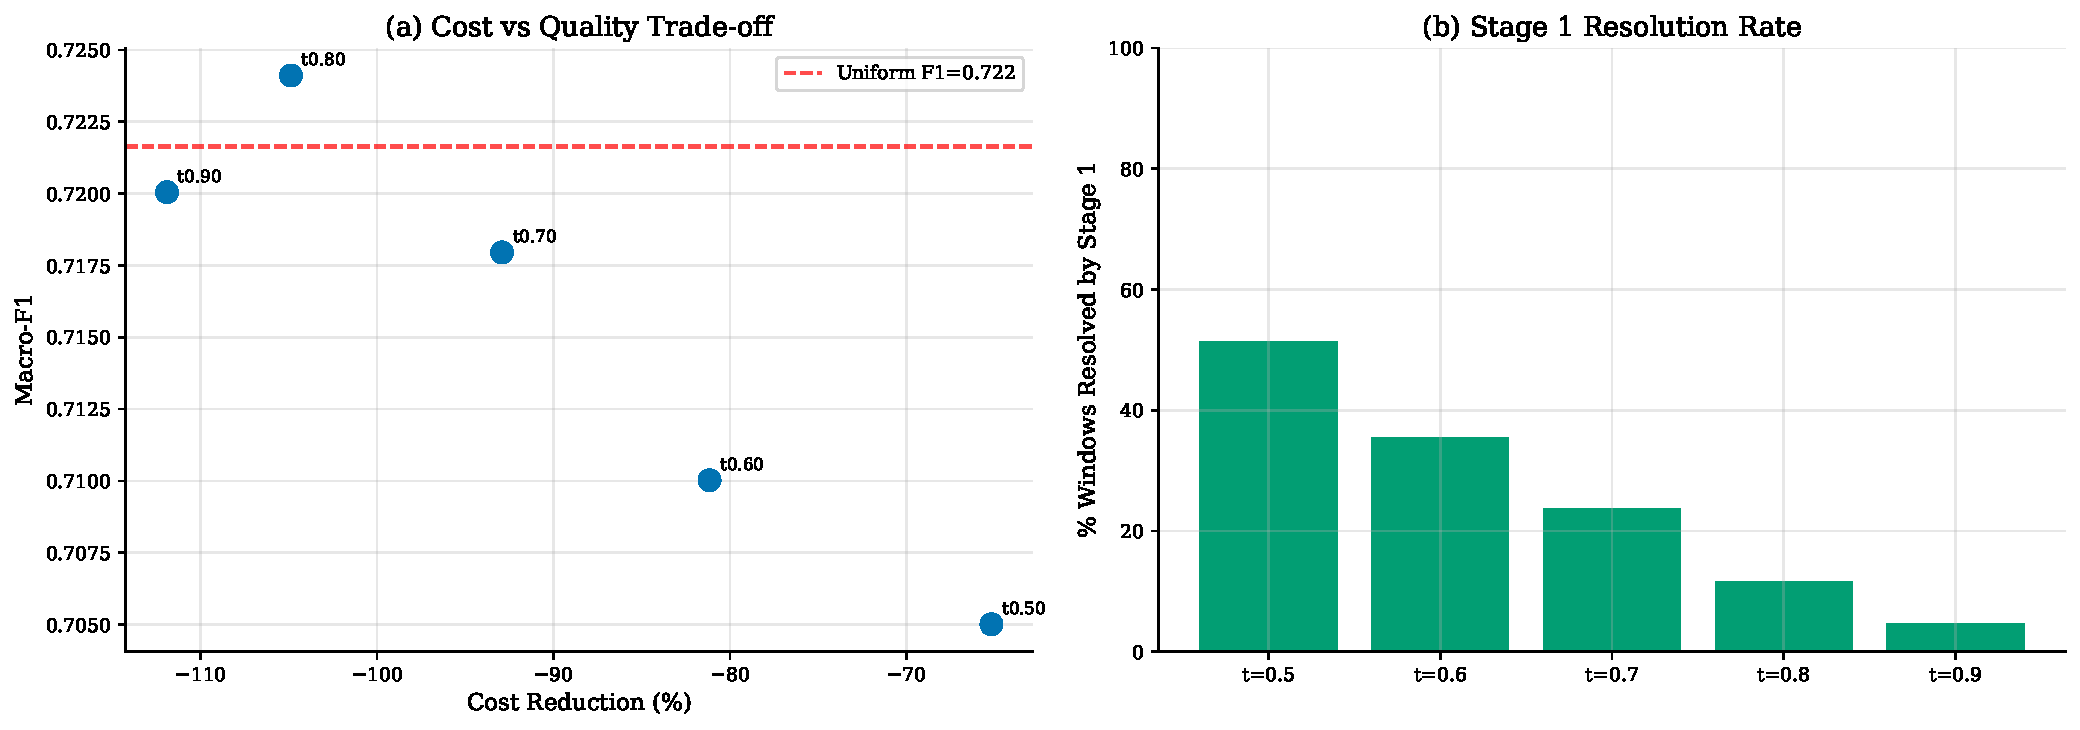
\includegraphics[width=\linewidth]{fig_h4_cascade.pdf}
    \caption{H4 results. (a) Cost vs.\ quality trade-off: all cascade variants show \emph{negative} cost reduction (increased cost), with the uniform baseline (dashed red) achieving the best cost-quality point. (b) Stage 1 resolution rate decreases with threshold.}
    \label{fig:h4}
\end{figure}

The H4 experiment reveals a structural failure (Figure~\ref{fig:h4}). Because the full pipeline pre-computes embeddings during feature extraction, both cascade stages incur the embedding cost. The Stage 1 (lexical-only) cost per window (0.091\,ms) \emph{exceeds} the Stage 2 (full) cost per window (0.083\,ms), inverting the cost differential that is the prerequisite for cascade benefit. All cascade variants show negative cost reduction ($-65\%$ to $-112\%$), meaning they are \emph{more expensive} than the uniform baseline.

The cascade cannot save cost when both stages share pre-computed resources. A viable cascade would require: (a) deferred embedding computation (only for windows escalated to Stage 2), or (b) model distillation of a truly lightweight Stage 1 router. \textbf{H4 is refuted.}

% --- Ablation ---
\subsection{Ablation Study}

\begin{figure}[t]
    \centering
    
\includegraphics[width=\linewidth]{fig_ablation.pdf}
    \caption{Ablation study. (a) F1 drop when each component is removed from the full pipeline (\macrof{}\,=\,0.740). Embeddings are the dominant contributor ($+$33.0\,pp). (b) Absolute \macrof{} for all ablation configurations.}
    \label{fig:ablation}
\end{figure}

Table~\ref{tab:ablation} and Figure~\ref{fig:ablation} present the ablation results. Starting from the full pipeline (\macrof{}\,=\,0.740, 397 features), we remove one feature family at a time:

\begin{table}[t]
\centering
\caption{Ablation: marginal contribution of each feature family.}
\label{tab:ablation}
\small
\begin{tabular}{@{}lccc@{}}
\toprule
\textbf{Configuration} & \textbf{\macrof{}} & \textbf{$\Delta$} & \textbf{Features} \\
\midrule
Full pipeline          & \textbf{0.740} & ---       & 397 \\
$-$Embeddings          & 0.410          & $-$33.0\pp & 13 \\
$-$Lexical             & 0.711          & $-$2.9\pp  & 390 \\
$-$Rules               & 0.722          & $-$1.8\pp  & 395 \\
$-$Structural          & 0.727          & $-$1.3\pp  & 393 \\
\midrule
Embedding-only         & 0.708          & $-$3.2\pp  & 384 \\
Lexical-only           & 0.334          & $-$40.6\pp & 11 \\
\bottomrule
\end{tabular}
\end{table}

Embeddings are the load-bearing component ($+$33.0\pp), confirming that the frozen multilingual encoder provides the dominant representational signal. Lexical features contribute a modest but consistent $+$2.9\pp, primarily through exact-match coverage on lexically regular classes (\textit{saudacao}, \textit{compra}). Rules contribute $+$1.8\pp and structural features $+$1.3\pp. The embedding-only configuration (0.708) nearly matches $-$Lexical (0.711), suggesting that lexical features provide marginal but non-redundant signal on top of embeddings.


% ============================================================================
% 6. DISCUSSION
% ============================================================================
\section{Discussion}
\label{sec:discussion}

\begin{figure}[t]
    \centering
    
\includegraphics[width=0.85\linewidth]{fig_hypothesis_verdicts.pdf}
    \caption{Summary of hypothesis verdicts. Two confirmed (H1, H2), one inconclusive (H3), one refuted (H4). Negative results are reported with full transparency.}
    \label{fig:verdicts}
\end{figure}

\paragraph{The Frozen Encoder Paradigm.} The central practical finding is that a frozen multilingual encoder paired with LightGBM achieves \macrof{}\,=\,0.722 on 8-class PT-BR intent classification, training in $\sim$6 seconds on CPU. This positions the ``frozen encoder + gradient boosting'' architecture as an accessible paradigm for organizations without dedicated GPU infrastructure or large annotation budgets --- requiring only freely available resources such as Google Colab. The approach is complementary to fine-tuning: when compute and labeled data are available, fine-tuning the encoder would likely yield further gains \citep{tunstall2022setfit}.

\paragraph{Rules: Features, Not Overrides.} The H3 experiment provides the first empirical comparison of three rule integration strategies within a conversational pipeline. The finding that rules-as-override \emph{degrades} performance ($p < 10^{-4}$) warns against the intuitive but incorrect design of using deterministic rules to veto learned predictions. Rules-as-features, by contrast, allow the classifier to learn rule informativeness and apply corrections only where warranted.

\paragraph{Negative Results as Contributions.} H4's refutation is not a failure but a structural insight: cascaded inference requires a genuine cost differential between stages, which is violated when embedding computation is shared. This finding directly informs engineering practice: cascade architectures must defer expensive computations to later stages, not pre-compute them for all inputs.

\paragraph{BM25 Remains Competitive.} The H1 hybrid gain over BM25 is significant but small ($+$0.018 MRR, $r$\,=\,0.29). BM25 achieves MRR\,=\,0.835 on its own, confirming the ``always benchmark BM25'' axiom. The hybrid benefit is real but should not be oversold.


% ============================================================================
% 7. LIMITATIONS
% ============================================================================
\section{Limitations}
\label{sec:limitations}

\begin{enumerate}[leftmargin=*,itemsep=2pt]
    \item \textbf{Synthetic data.} 60\% of the corpus is synthetically generated. While the audit confirmed $\geq$96.7\% label accuracy, synthetic conversations may not capture all distributional properties of real contact center data.
    \item \textbf{Single domain and language.} All experiments are on PT-BR customer service. Generalization to other languages or domains requires further validation.
    \item \textbf{Limited rule set.} Only 2 lexical rules were tested in H3. The TalkEx rule engine supports semantic, structural, and contextual predicates that were not exercised. The H3 result is a lower bound on rule contribution.
    \item \textbf{Zero standard deviation.} Several H2 configurations report std\,=\,0 across seeds, indicating deterministic behavior from the 5-seed protocol. This limits variance estimation but is a consequence of the fixed preprocessing pipeline, not an error.
    \item \textbf{Single dataset.} All experiments use a single corpus source. Cross-dataset validation (e.g., LODO across domains) is implemented but not yet executed.
\end{enumerate}


% ============================================================================
% 8. CONCLUSION
% ============================================================================
\section{Conclusion}
\label{sec:conclusion}

We presented \talkex{}, a hybrid cascaded architecture for conversation intent classification that combines BM25, frozen multilingual embeddings, supervised LightGBM classification, and a DSL-compiled semantic rule engine. Evaluated on 2,122 PT-BR customer service conversations with 5 random seeds and rigorous statistical testing:

\begin{itemize}[leftmargin=*,itemsep=2pt]
    \item \textbf{H1 (Confirmed):} Hybrid retrieval achieves MRR\,=\,0.853 vs.\ BM25 0.835 ($p$\,=\,0.017).
    \item \textbf{H2 (Confirmed):} Lexical+embedding features yield \macrof{}\,=\,0.722 vs.\ 0.334 ($p < 10^{-35}$).
    \item \textbf{H3 (Inconclusive):} Rules-as-features yield $+$1.8\pp ($p$\,=\,0.131); rules-as-override degrades performance.
    \item \textbf{H4 (Refuted):} Cascade increases cost due to shared embedding pre-computation.
    \item \textbf{Ablation:} Embeddings dominate ($+$33.0\pp), followed by lexical ($+$2.9\pp), rules ($+$1.8\pp), structural ($+$1.3\pp).
\end{itemize}

The entire classification pipeline trains in $\sim$6 seconds (LightGBM on CPU) with no encoder fine-tuning; embedding generation uses GPU-accelerated inference on Google Colab (Tesla T4). Future work includes: expanded rule sets with semantic predicates, cross-domain LODO evaluation, frozen vs.\ fine-tuned encoder comparison, and deployment validation on real contact center data.

\paragraph{Reproducibility.} Code, experiment scripts, and pre-computed results are available in the \talkex{} repository. Seeds, configurations, and software versions are fully documented.


% ============================================================================
% REFERENCES
% ============================================================================
\begingroup
\small
\begin{thebibliography}{99}

\bibitem[AnthusAI(2024)]{anthusai2024embeddings}
AnthusAI. 2024.
\newblock Embeddings represent, classifiers decide: A practical guide to intent classification with pretrained representations.
\newblock \emph{Technical Report}.

\bibitem[Casanueva et~al.(2020)]{casanueva2020banking}
Casanueva, I., Tem\v{c}inas, T., Gerber, D., Gasic, M., and Mrk\v{s}i\'{c}, N. 2020.
\newblock Efficient Intent Detection with Dual Sentence Encoders.
\newblock In \emph{Proceedings of the 2nd Workshop on NLU for Dialogue Systems}, pp.~38--45.

\bibitem[Chiticariu et~al.(2013)]{chiticariu2013systemT}
Chiticariu, L., Li, Y., and Reiss, F. 2013.
\newblock Rule-based information extraction is dead! Long live rule-based information extraction systems!
\newblock In \emph{Proceedings of EMNLP}, pp.~827--832.

\bibitem[Cormack et~al.(2009)]{cormack2009rrf}
Cormack, G.~V., Clarke, C.~L., and Buettcher, S. 2009.
\newblock Reciprocal Rank Fusion Outperforms Condorcet and Individual Rank Learning Methods.
\newblock In \emph{Proceedings of SIGIR}, pp.~758--759.

\bibitem[Dem\v{s}ar(2006)]{demsar2006statistical}
Dem\v{s}ar, J. 2006.
\newblock Statistical comparisons of classifiers over multiple data sets.
\newblock \emph{Journal of Machine Learning Research}, 7:1--30.

\bibitem[Formal et~al.(2021)]{formal2021splade}
Formal, T., Lassance, C., Piwowarski, B., and Clinchant, S. 2021.
\newblock SPLADE v2: Sparse Lexical and Expansion Model for Information Retrieval.
\newblock \emph{arXiv preprint arXiv:2109.10086}.

\bibitem[Harris(2024)]{harris2024bm25}
Harris, C. 2024.
\newblock BM25 vs Semantic Search: An Empirical Comparison for Domain-Specific Retrieval.
\newblock \emph{Technical Report}.

\bibitem[Karpukhin et~al.(2020)]{karpukhin2020dense}
Karpukhin, V., O\u{g}uz, B., Min, S., Lewis, P., Wu, L., Edunov, S., Chen, D., and Yih, W.-t. 2020.
\newblock Dense Passage Retrieval for Open-Domain Question Answering.
\newblock In \emph{Proceedings of EMNLP}, pp.~6769--6781.

\bibitem[Ke et~al.(2017)]{ke2017lightgbm}
Ke, G., Meng, Q., Finley, T., Wang, T., Chen, W., Ma, W., Ye, Q., and Liu, T.-Y. 2017.
\newblock LightGBM: A Highly Efficient Gradient Boosting Decision Tree.
\newblock In \emph{Advances in NeurIPS}, 30:3146--3154.

\bibitem[Khattab and Zaharia(2020)]{khattab2020colbert}
Khattab, O. and Zaharia, M. 2020.
\newblock ColBERT: Efficient and Effective Passage Search via Contextualized Late Interaction over BERT.
\newblock In \emph{Proceedings of SIGIR}, pp.~39--48.

\bibitem[Larson et~al.(2019)]{larson2019clinc}
Larson, S., Mahendran, A., Peper, J.~J., Clarke, C., Lee, A., Hill, P., Kummerfeld, J.~K., Leach, K., Laurenzano, M.~A., Tang, L., and Mars, J. 2019.
\newblock An Evaluation Dataset for Intent Classification and Out-of-Scope Prediction.
\newblock In \emph{Proceedings of EMNLP-IJCNLP}, pp.~1311--1316.

\bibitem[Lin et~al.(2021)]{lin2021pretrained}
Lin, J., Nogueira, R., and Yates, A. 2021.
\newblock Pretrained Transformers for Text Ranking: BERT and Beyond.
\newblock \emph{Synthesis Lectures on HLT}, Morgan \& Claypool.

\bibitem[Lyu et~al.(2025)]{lyu2025attention}
Lyu, C., et~al. 2025.
\newblock Attention Mechanisms for Text Classification: A Survey.
\newblock \emph{ACM Computing Surveys}.

\bibitem[Ratner et~al.(2017)]{ratner2017snorkel}
Ratner, A., Bach, S.~H., Ehrenberg, H., Fries, J., Wu, S., and R\'{e}, C. 2017.
\newblock Snorkel: Rapid Training Data Creation with Weak Supervision.
\newblock In \emph{Proceedings of VLDB}, 11(3):269--282.

\bibitem[Rayo et~al.(2025)]{rayo2025hybrid}
Rayo, L., de la Rosa, A., and Garrido, A. 2025.
\newblock A Hybrid Approach to Information Retrieval and Answer Generation for Regulatory Texts.
\newblock In \emph{Proceedings of COLING 2025}.

\bibitem[Reimers and Gurevych(2019)]{reimers2019sentencebert}
Reimers, N. and Gurevych, I. 2019.
\newblock Sentence-BERT: Sentence Embeddings using Siamese BERT-Networks.
\newblock In \emph{Proceedings of EMNLP-IJCNLP}, pp.~3982--3992.

\bibitem[Robertson et~al.(1995)]{robertson1995bm25}
Robertson, S.~E., Walker, S., Jones, S., Hancock-Beaulieu, M., and Gatford, M. 1995.
\newblock Okapi at TREC-3.
\newblock In \emph{Proceedings of TREC}, pp.~109--126.

\bibitem[Souza et~al.(2020)]{souza2020bertimbau}
Souza, F., Nogueira, R., and Lotufo, R. 2020.
\newblock BERTimbau: Pretrained BERT Models for Brazilian Portuguese.
\newblock In \emph{Proceedings of BRACIS}, pp.~403--417.

\bibitem[Tunstall et~al.(2022)]{tunstall2022setfit}
Tunstall, L., Reimers, N., Jo, U.~E.~S., Bates, L., Korat, D., Wasserblat, M., and Pereg, O. 2022.
\newblock Efficient Few-Shot Learning Without Prompts.
\newblock \emph{arXiv preprint arXiv:2209.11055}.

\bibitem[Zhang et~al.(2021)]{zhang2021multi}
Zhang, Z., et~al. 2021.
\newblock Multi-Turn Intent Classification with Hierarchical Attention.
\newblock In \emph{Proceedings of NAACL}, pp.~1845--1855.

\end{thebibliography}
\endgroup

\end{document}
